
%% bare_conf.tex
%% V1.3
%% 2007/01/11
%% by Michael Shell
%% See:
%% http://www.michaelshell.org/
%% for current contact information.
%%
%% This is a skeleton file demonstrating the use of IEEEtran.cls
%% (requires IEEEtran.cls version 1.7 or later) with an IEEE conference paper.
%%
%% Support sites:
%% http://www.michaelshell.org/tex/ieeetran/
%% http://www.ctan.org/tex-archive/macros/latex/contrib/IEEEtran/
%% and
%% http://www.ieee.org/

%%*************************************************************************
%% Legal Notice:
%% This code is offered as-is without any warranty either expressed or
%% implied; without even the implied warranty of MERCHANTABILITY or
%% FITNESS FOR A PARTICULAR PURPOSE! 
%% User assumes all risk.
%% In no event shall IEEE or any contributor to this code be liable for
%% any damages or losses, including, but not limited to, incidental,
%% consequential, or any other damages, resulting from the use or misuse
%% of any information contained here.
%%
%% All comments are the opinions of their respective authors and are not
%% necessarily endorsed by the IEEE.
%%
%% This work is distributed under the LaTeX Project Public License (LPPL)
%% ( http://www.latex-project.org/ ) version 1.3, and may be freely used,
%% distributed and modified. A copy of the LPPL, version 1.3, is included
%% in the base LaTeX documentation of all distributions of LaTeX released
%% 2003/12/01 or later.
%% Retain all contribution notices and credits.
%% ** Modified files should be clearly indicated as such, including  **
%% ** renaming them and changing author support contact information. **
%%
%% File list of work: IEEEtran.cls, IEEEtran_HOWTO.pdf, bare_adv.tex,
%%                    bare_conf.tex, bare_jrnl.tex, bare_jrnl_compsoc.tex
%%*************************************************************************

% *** Authors should verify (and, if needed, correct) their LaTeX system  ***
% *** with the testflow diagnostic prior to trusting their LaTeX platform ***
% *** with production work. IEEE's font choices can trigger bugs that do  ***
% *** not appear when using other class files.                            ***
% The testflow support page is at:
% http://www.michaelshell.org/tex/testflow/



% Note that the a4paper option is mainly intended so that authors in
% countries using A4 can easily print to A4 and see how their papers will
% look in print - the typesetting of the document will not typically be
% affected with changes in paper size (but the bottom and side margins will).
% Use the testflow package mentioned above to verify correct handling of
% both paper sizes by the user's LaTeX system.
%
% Also note that the "draftcls" or "draftclsnofoot", not "draft", option
% should be used if it is desired that the figures are to be displayed in
% draft mode.
%
\documentclass[10pt, conference, compsocconf]{IEEEtran}
\usepackage[pdftex]{graphicx}
\usepackage{cite}
\usepackage[cmex10]{amsmath}
\usepackage{algorithmic}
\usepackage{url}
\usepackage{mdwmath}
\usepackage{mdwtab}


% Add the compsocconf option for Computer Society conferences.
%
% If IEEEtran.cls has not been installed into the LaTeX system files,
% manually specify the path to it like:
% \documentclass[conference]{../sty/IEEEtran}





% Some very useful LaTeX packages include:
% (uncomment the ones you want to load)


% *** MISC UTILITY PACKAGES ***
%
%\usepackage{ifpdf}
% Heiko Oberdiek's ifpdf.sty is very useful if you need conditional
% compilation based on whether the output is pdf or dvi.
% usage:
% \ifpdf
%   % pdf code
% \else
%   % dvi code
% \fi
% The latest version of ifpdf.sty can be obtained from:
% http://www.ctan.org/tex-archive/macros/latex/contrib/oberdiek/
% Also, note that IEEEtran.cls V1.7 and later provides a builtin
% \ifCLASSINFOpdf conditional that works the same way.
% When switching from latex to pdflatex and vice-versa, the compiler may
% have to be run twice to clear warning/error messages.






% *** CITATION PACKAGES ***
%
%\usepackage{cite}
% cite.sty was written by Donald Arseneau
% V1.6 and later of IEEEtran pre-defines the format of the cite.sty package
% \cite{} output to follow that of IEEE. Loading the cite package will
% result in citation numbers being automatically sorted and properly
% "compressed/ranged". e.g., [1], [9], [2], [7], [5], [6] without using
% cite.sty will become [1], [2], [5]--[7], [9] using cite.sty. cite.sty's
% \cite will automatically add leading space, if needed. Use cite.sty's
% noadjust option (cite.sty V3.8 and later) if you want to turn this off.
% cite.sty is already installed on most LaTeX systems. Be sure and use
% version 4.0 (2003-05-27) and later if using hyperref.sty. cite.sty does
% not currently provide for hyperlinked citations.
% The latest version can be obtained at:
% http://www.ctan.org/tex-archive/macros/latex/contrib/cite/
% The documentation is contained in the cite.sty file itself.






% *** GRAPHICS RELATED PACKAGES ***
%
\ifCLASSINFOpdf
  % \usepackage[pdftex]{graphicx}
  % declare the path(s) where your graphic files are
  % \graphicspath{{../pdf/}{../jpeg/}}
  % and their extensions so you won't have to specify these with
  % every instance of \includegraphics
  % \DeclareGraphicsExtensions{.pdf,.jpeg,.png}
\else
  % or other class option (dvipsone, dvipdf, if not using dvips). graphicx
  % will default to the driver specified in the system graphics.cfg if no
  % driver is specified.
  % \usepackage[dvips]{graphicx}
  % declare the path(s) where your graphic files are
  % \graphicspath{{../eps/}}
  % and their extensions so you won't have to specify these with
  % every instance of \includegraphics
  % \DeclareGraphicsExtensions{.eps}
\fi
% graphicx was written by David Carlisle and Sebastian Rahtz. It is
% required if you want graphics, photos, etc. graphicx.sty is already
% installed on most LaTeX systems. The latest version and documentation can
% be obtained at: 
% http://www.ctan.org/tex-archive/macros/latex/required/graphics/
% Another good source of documentation is "Using Imported Graphics in
% LaTeX2e" by Keith Reckdahl which can be found as epslatex.ps or
% epslatex.pdf at: http://www.ctan.org/tex-archive/info/
%
% latex, and pdflatex in dvi mode, support graphics in encapsulated
% postscript (.eps) format. pdflatex in pdf mode supports graphics
% in .pdf, .jpeg, .png and .mps (metapost) formats. Users should ensure
% that all non-photo figures use a vector format (.eps, .pdf, .mps) and
% not a bitmapped formats (.jpeg, .png). IEEE frowns on bitmapped formats
% which can result in "jaggedy"/blurry rendering of lines and letters as
% well as large increases in file sizes.
%
% You can find documentation about the pdfTeX application at:
% http://www.tug.org/applications/pdftex





% *** MATH PACKAGES ***
%
%\usepackage[cmex10]{amsmath}
% A popular package from the American Mathematical Society that provides
% many useful and powerful commands for dealing with mathematics. If using
% it, be sure to load this package with the cmex10 option to ensure that
% only type 1 fonts will utilized at all point sizes. Without this option,
% it is possible that some math symbols, particularly those within
% footnotes, will be rendered in bitmap form which will result in a
% document that can not be IEEE Xplore compliant!
%
% Also, note that the amsmath package sets \interdisplaylinepenalty to 10000
% thus preventing page breaks from occurring within multiline equations. Use:
%\interdisplaylinepenalty=2500
% after loading amsmath to restore such page breaks as IEEEtran.cls normally
% does. amsmath.sty is already installed on most LaTeX systems. The latest
% version and documentation can be obtained at:
% http://www.ctan.org/tex-archive/macros/latex/required/amslatex/math/





% *** SPECIALIZED LIST PACKAGES ***
%
%\usepackage{algorithmic}
% algorithmic.sty was written by Peter Williams and Rogerio Brito.
% This package provides an algorithmic environment fo describing algorithms.
% You can use the algorithmic environment in-text or within a figure
% environment to provide for a floating algorithm. Do NOT use the algorithm
% floating environment provided by algorithm.sty (by the same authors) or
% algorithm2e.sty (by Christophe Fiorio) as IEEE does not use dedicated
% algorithm float types and packages that provide these will not provide
% correct IEEE style captions. The latest version and documentation of
% algorithmic.sty can be obtained at:
% http://www.ctan.org/tex-archive/macros/latex/contrib/algorithms/
% There is also a support site at:
% http://algorithms.berlios.de/index.html
% Also of interest may be the (relatively newer and more customizable)
% algorithmicx.sty package by Szasz Janos:
% http://www.ctan.org/tex-archive/macros/latex/contrib/algorithmicx/




% *** ALIGNMENT PACKAGES ***
%
%\usepackage{array}
% Frank Mittelbach's and David Carlisle's array.sty patches and improves
% the standard LaTeX2e array and tabular environments to provide better
% appearance and additional user controls. As the default LaTeX2e table
% generation code is lacking to the point of almost being broken with
% respect to the quality of the end results, all users are strongly
% advised to use an enhanced (at the very least that provided by array.sty)
% set of table tools. array.sty is already installed on most systems. The
% latest version and documentation can be obtained at:
% http://www.ctan.org/tex-archive/macros/latex/required/tools/


%\usepackage{mdwmath}
%\usepackage{mdwtab}
% Also highly recommended is Mark Wooding's extremely powerful MDW tools,
% especially mdwmath.sty and mdwtab.sty which are used to format equations
% and tables, respectively. The MDWtools set is already installed on most
% LaTeX systems. The lastest version and documentation is available at:
% http://www.ctan.org/tex-archive/macros/latex/contrib/mdwtools/


% IEEEtran contains the IEEEeqnarray family of commands that can be used to
% generate multiline equations as well as matrices, tables, etc., of high
% quality.


%\usepackage{eqparbox}
% Also of notable interest is Scott Pakin's eqparbox package for creating
% (automatically sized) equal width boxes - aka "natural width parboxes".
% Available at:
% http://www.ctan.org/tex-archive/macros/latex/contrib/eqparbox/



% *** SUBFIGURE PACKAGES ***
%\usepackage[tight,footnotesize]{subfigure}
% subfigure.sty was written by Steven Douglas Cochran. This package makes it
% easy to put subfigures in your figures. e.g., "Figure 1a and 1b". For IEEE
% work, it is a good idea to load it with the tight package option to reduce
% the amount of white space around the subfigures. subfigure.sty is already
% installed on most LaTeX systems. The latest version and documentation can
% be obtained at:
% http://www.ctan.org/tex-archive/obsolete/macros/latex/contrib/subfigure/
% subfigure.sty has been superceeded by subfig.sty.



%\usepackage[caption=false]{caption}
%\usepackage[font=footnotesize]{subfig}
% subfig.sty, also written by Steven Douglas Cochran, is the modern
% replacement for subfigure.sty. However, subfig.sty requires and
% automatically loads Axel Sommerfeldt's caption.sty which will override
% IEEEtran.cls handling of captions and this will result in nonIEEE style
% figure/table captions. To prevent this problem, be sure and preload
% caption.sty with its "caption=false" package option. This is will preserve
% IEEEtran.cls handing of captions. Version 1.3 (2005/06/28) and later 
% (recommended due to many improvements over 1.2) of subfig.sty supports
% the caption=false option directly:
%\usepackage[caption=false,font=footnotesize]{subfig}
%
% The latest version and documentation can be obtained at:
% http://www.ctan.org/tex-archive/macros/latex/contrib/subfig/
% The latest version and documentation of caption.sty can be obtained at:
% http://www.ctan.org/tex-archive/macros/latex/contrib/caption/




% *** FLOAT PACKAGES ***
%
%\usepackage{fixltx2e}
% fixltx2e, the successor to the earlier fix2col.sty, was written by
% Frank Mittelbach and David Carlisle. This package corrects a few problems
% in the LaTeX2e kernel, the most notable of which is that in current
% LaTeX2e releases, the ordering of single and double column floats is not
% guaranteed to be preserved. Thus, an unpatched LaTeX2e can allow a
% single column figure to be placed prior to an earlier double column
% figure. The latest version and documentation can be found at:
% http://www.ctan.org/tex-archive/macros/latex/base/



%\usepackage{stfloats}
% stfloats.sty was written by Sigitas Tolusis. This package gives LaTeX2e
% the ability to do double column floats at the bottom of the page as well
% as the top. (e.g., "\begin{figure*}[!b]" is not normally possible in
% LaTeX2e). It also provides a command:
%\fnbelowfloat
% to enable the placement of footnotes below bottom floats (the standard
% LaTeX2e kernel puts them above bottom floats). This is an invasive package
% which rewrites many portions of the LaTeX2e float routines. It may not work
% with other packages that modify the LaTeX2e float routines. The latest
% version and documentation can be obtained at:
% http://www.ctan.org/tex-archive/macros/latex/contrib/sttools/
% Documentation is contained in the stfloats.sty comments as well as in the
% presfull.pdf file. Do not use the stfloats baselinefloat ability as IEEE
% does not allow \baselineskip to stretch. Authors submitting work to the
% IEEE should note that IEEE rarely uses double column equations and
% that authors should try to avoid such use. Do not be tempted to use the
% cuted.sty or midfloat.sty packages (also by Sigitas Tolusis) as IEEE does
% not format its papers in such ways.





% *** PDF, URL AND HYPERLINK PACKAGES ***
%
%\usepackage{url}
% url.sty was written by Donald Arseneau. It provides better support for
% handling and breaking URLs. url.sty is already installed on most LaTeX
% systems. The latest version can be obtained at:
% http://www.ctan.org/tex-archive/macros/latex/contrib/misc/
% Read the url.sty source comments for usage information. Basically,
% \url{my_url_here}.





% *** Do not adjust lengths that control margins, column widths, etc. ***
% *** Do not use packages that alter fonts (such as pslatex).         ***
% There should be no need to do such things with IEEEtran.cls V1.6 and later.
% (Unless specifically asked to do so by the journal or conference you plan
% to submit to, of course. )


% correct bad hyphenation here
\hyphenation{op-tical net-works semi-conduc-tor}


\begin{document}
%
% paper title
% can use linebreaks \\ within to get better formatting as desired
\title{Energy Aggregation using Product of Experts}


% author names and affiliations
% use a multiple column layout for up to two different
% affiliations

\author{\IEEEauthorblockN{Dr. Haimonti Dutta}
\IEEEauthorblockA{Center for Computational Learning System,\\
Columbia University\\
New York, NY 10115\\
haimonti@ccls.columbia.edu}
\and
\IEEEauthorblockN{Megha Gupta}
\IEEEauthorblockA{Dept. of Computer Science,\\
IIIT-D\\
Delhi, India.\\
meghag@iiitd.ac.in}
}

% conference papers do not typically use \thanks and this command
% is locked out in conference mode. If really needed, such as for
% the acknowledgment of grants, issue a \IEEEoverridecommandlockouts
% after \documentclass

% for over three affiliations, or if they all won't fit within the width
% of the page, use this alternative format:
% 
%\author{\IEEEauthorblockN{Michael Shell\IEEEauthorrefmark{1},
%Homer Simpson\IEEEauthorrefmark{2},
%James Kirk\IEEEauthorrefmark{3}, 
%Montgomery Scott\IEEEauthorrefmark{3} and
%Eldon Tyrell\IEEEauthorrefmark{4}}
%\IEEEauthorblockA{\IEEEauthorrefmark{1}School of Electrical and Computer Engineering\\
%Georgia Institute of Technology,
%Atlanta, Georgia 30332--0250\\ Email: see http://www.michaelshell.org/contact.html}
%\IEEEauthorblockA{\IEEEauthorrefmark{2}Twentieth Century Fox, Springfield, USA\\
%Email: homer@thesimpsons.com}
%\IEEEauthorblockA{\IEEEauthorrefmark{3}Starfleet Academy, San Francisco, California 96678-2391\\
%Telephone: (800) 555--1212, Fax: (888) 555--1212}
%\IEEEauthorblockA{\IEEEauthorrefmark{4}Tyrell Inc., 123 Replicant Street, Los Angeles, California 90210--4321}}




% use for special paper notices
%\IEEEspecialpapernotice{(Invited Paper)}




% make the title area
\maketitle


\begin{abstract}
The abstract goes here. DO NOT USE SPECIAL CHARACTERS, SYMBOLS, OR MATH IN YOUR TITLE OR ABSTRACT.

\end{abstract}

\begin{IEEEkeywords}
product of experts; energy aggregation; contrastive divergence;

\end{IEEEkeywords}


% For peer review papers, you can put extra information on the cover
% page as needed:
% \ifCLASSOPTIONpeerreview
% \begin{center} \bfseries EDICS Category: 3-BBND \end{center}
% \fi
%
% For peerreview papers, this IEEEtran command inserts a page break and
% creates the second title. It will be ignored for other modes.
\IEEEpeerreviewmaketitle



\section{Introduction}
% no \IEEEPARstart

% You must have at least 2 lines in the paragraph with the drop letter
% (should never be an issue)

\section{Related Work}
\subsection{Automata and their products}
\label{sec:related}

Distributed networks can be modelled using interacting automata. Benveniste defines automaton as a quadruple, \'{A} = (X,X$_{0}$,A,T) where X is a finite state of sets, X0 is the subset of initial states, A is a finite set of messages, T is a set of transitions of the form t = \{x\_,a,x\} where x\_ is the previous state, a is the message label on which the state transitions to the next state x. The figure~\ref{fig:ex} below explains the automata with an example.\\

\begin{figure*}[t]
\centering
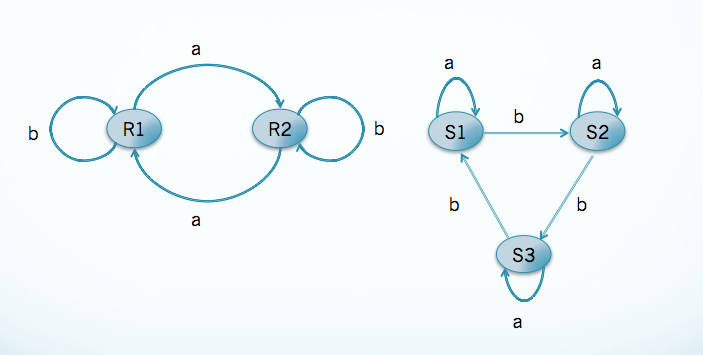
\includegraphics[width=8cm,height=3cm]{automata.png}
\caption{Automata R and S}
\label{fig:ex}
\end{figure*}

For automaton R, X$_{R}$ = \{2; R1,R2\}, X$_{0R}$ = \{R1\}, A$_{R}$ = \{a,b\}, T$_{R}$ = \{R1,a,R1; R1,b,R2; R2,a,R2; R2,b,R1\} \\
For automaton S, X$_{S}$ = \{3; S1,S2,S3\}, X$_{0S}$ = \{S1\}, A$_{S}$ = \{a,b\}, T$_{S}$ = \{S1,a,S1; S1,b,S2; S2,a,S2; S2,b,S3; S3,a,S3; S3,b,S1\} \\
The product of two automata \'{A} = R x S is defined as follows: \\
X = X$_{R}$ x X$_{S}$ \\
X$_{0}$ = X$_{0R}$ x X$_{0S}$ \\
A = A$_{R}$ $\cup$ A$_{S}$ \\
%t = (x\_,a,x)  \\
Benveniste uses a notion of stuttering transition which helps to distinguish between local and global time by inserting dummy transitions between two transitions of a local automaton attached to a node. This stuttering transition does nothing but lets the rest of the world progress.

\begin{table}[h]
\centering
\begin{tabular}{ l | c | c }
 A & R1 & R2 \\
\hline
R1 & 0.6 & 0.4 \\
R2 & 0.3 & 0.7 \\
\end{tabular}
\caption{Transition probability, A}
\label{table:A}
\end{table}

\begin{table}[h]
\centering
\begin{tabular}{ l | c | c }
 B & a & b \\
\hline
R1 & 0.2 & 0.8 \\
R2 & 0.5 & 0.5 \\
\end{tabular}
\caption{Observed probability, B}
\label{table:B}
\end{table}

\begin{table}[h]
\centering
\begin{tabular}{ l | c | c }
&  R1 & R2 \\
\hline
$\pi$ & 0.4 & 0.6 \\

\end{tabular}
\caption{Initial state probability, $\pi$}
\label{table:pi}
\end{table}

Talking in terms of HMM, requires us to equip products of automata with probabilities. Benveniste defines HMM as a triple (\'{A}, $\mu$, $\pi$) where \'{A} = (X,X$_{0}$,A,T) is an automaton, $\mu$ is the initial state probability, $\pi$ is factored as state transition probability $\pi$$_{x}$ and message transition probability $\pi$$_{A}$. He uses a random arbiter $\alpha$, with values {first, second, third} to choose automaton to initiate transition. If $\alpha$ = first then first automaton chooses any transition having a private message whereas second automaton performs a stuttering transition, and vice versa for $\alpha$ = second. If $\alpha$ = both, then both automata agree on some shared message and move accordingly.

Using the traditional HMM notation of the parameters $\lambda$ = \{A, B, $\pi$ \} where A is the transition probability, B is the observed probability, $\pi$ is the initial state probability. For automata R, we have the values of A, B, $\pi$ as shown in table ~\ref{table:A}, ~\ref{table:B}, ~\ref{table:pi} respectively.

\subsection{Product of HMM}
\label {sec:pohmm}
Product of HMM is a way of combining HMM's to form distributed state time series model. The figure~\ref{fig:pohmm} is a product of two HMMs shown in~\ref{fig:ex}. For  P = R x S, the quadruple becomes\\
X = \{6; R1S1, R1S2, R1S3, R2S1, R2S2, R2S3\} \\
X$_{0}$ = \{R1S1\} \\
A = \{a,b\} \\
The rules for synchronised product construction are : \\
1. $<p,q>$ --a--$>$ $<p',q>$ if a $\in$ A$_{R}$ $\cap$ A$_{S}$ and p --a--$>$ p' and q --a--$>$ q'	\\
2. $<p,q>$ --a--$>$ $<p',q>$ if a $\in$ A$_{R}$, a $\notin$ A$_{S}$ and p --a--$>$ p'	\\
3. $<p,q>$ --a--$>$ $<p,q'>$ if a $\notin$ A$_{R}$, a $\in$ A$_{S}$ and q --a--$>$ q'	\\

\begin{figure*}[t]
\centering
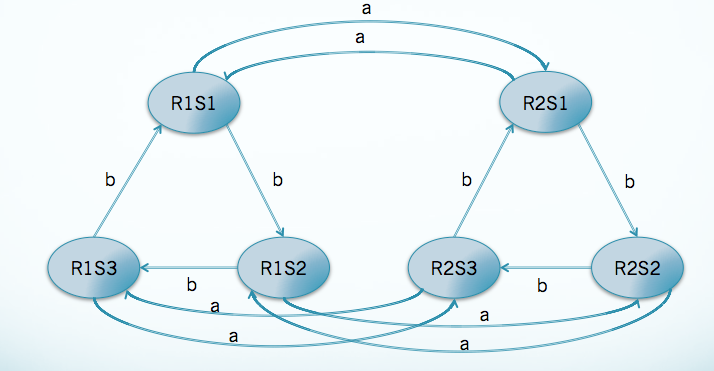
\includegraphics[width=8cm,height=3cm]{product.png}
\caption{Product of HMMs, P = R x S}
\label{fig:pohmm}
\end{figure*}


\section{Methodology}
\subsection{Training product of experts by minimising contrastive divergence}
High dimensional distributions are approximated as a product of one dimensional distributions. The product of individual distributions which is uniguassian or multivariate guassian will also be multivariate guassian. If the individual models are more complicated and contain one or more hidden variables, multiplying their distributions together and renormalizing them can be very powerful. These individual models are called "experts".
The product of experts produce sharper distribution than the individual distributions\cite{hinton2000}.

\section{Proof of concept on REDD House 2}
%\begin{enumerate}
\subsection{Aim}
 To represent streams of energy consumption data from $n$\footnote{n=2} appliances by product(s) of $k$ HMMs.
 
\subsection{Method} 

\begin{itemize}
\item \textbf{Data } The Reference Energy Disaggregation Data Set (REDD) is used in empirical analysis. The data contains power consumption from real homes, for the whole house as well as for each individual circuit in
the house (labeled by the main type of appliance on that circuit). It is intended for use in developing disaggregation methods, which can predict, from only the whole-home signal, which devices are being used. The REDD data set contains two main types of home electricity data: high-frequency current/voltage waveform data of the two power mains (as well as the voltage signal for a single phase), and lower-frequency power data including the mains and individual, labeled circuits in the house. The main directory consists of several house\_i directories, each of which contain all the power readings for a single house.  Each house subdirectory consists of a labels.dat and several channels\_i.dat files. The labels file contains channel numbers and a text label indicating the general category of device on this channel. Each channel\_i.dat file has two columns containing UTC timestamps (as integers) and power readings (recording the apparent power of the circuit) for the channel.
Experiments reported here use the House 2 data from REDD. It has $11$ channels where each channel corresponds to the following appliance: 
\begin{enumerate}
\item mains$\_1$ 
\item mains$\_2$ 
\item kitchen$\_$1
\item lighting
\item stove 
\item microwave
\item washer$\_$dryer
\item kitchen$\_2$
\item refrigerator
\item dishwaser
\item disposal
\end{enumerate}

The dataset has $318759$ records and $2$ columns. We randomly sample 300 records for our experiment. Time series data from two appliances are represented as product of $k$ HMMs.


\item \textbf{ Time Series :} The time series data of the microwave, dryer, kitchen$\_2$ and refrigerator are plotted below in Figures~\ref{fig:micro}, ~\ref{fig:washer}, ~\ref{fig:kitchen2}, ~\ref{fig:refri}.

%\begin{figure*}[!t]
%\centerline{\subfloat[Case I]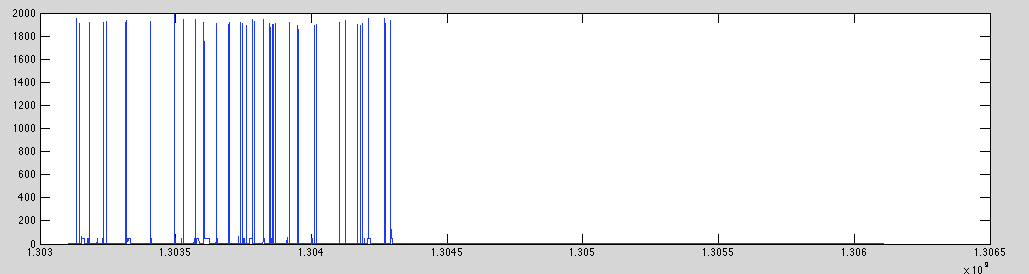
\includegraphics[width=1.0]{channel_6.png}
%\label{fig:micro}}
%\hfil
%\subfloat[Case II]{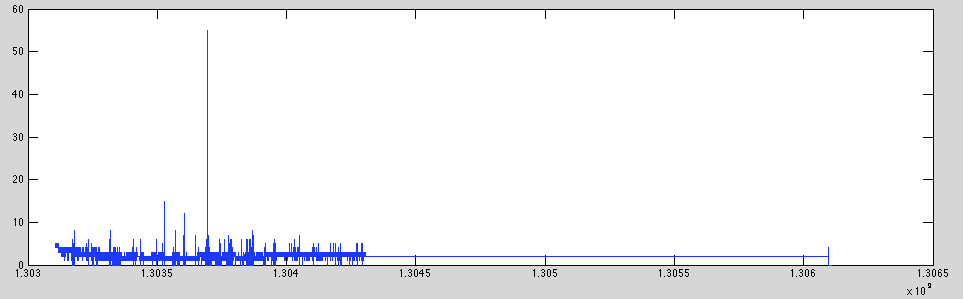
\includegraphics[width=1.0]{channel_7.png}
%\label{fig:washer}}}
%\caption{Simulation results}
%\label{fig:washer}
%\end{figure*}

\begin{figure*}[t]
\centering
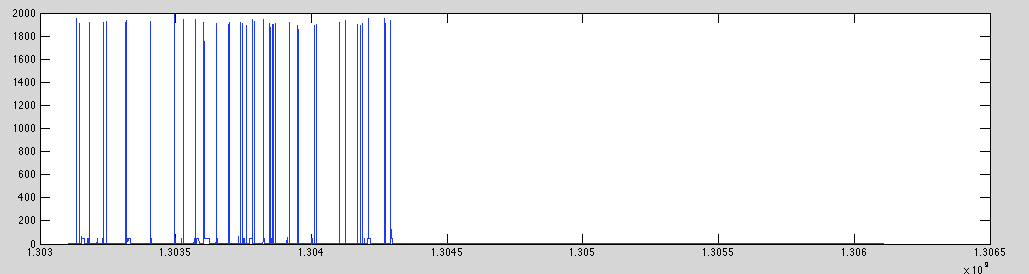
\includegraphics[width=1.0\textwidth,height=0.15\textheight]{channel_6.png}
\caption{Microwave}
\label{fig:micro}
\end{figure*}

\begin{figure*}[t]
\centering
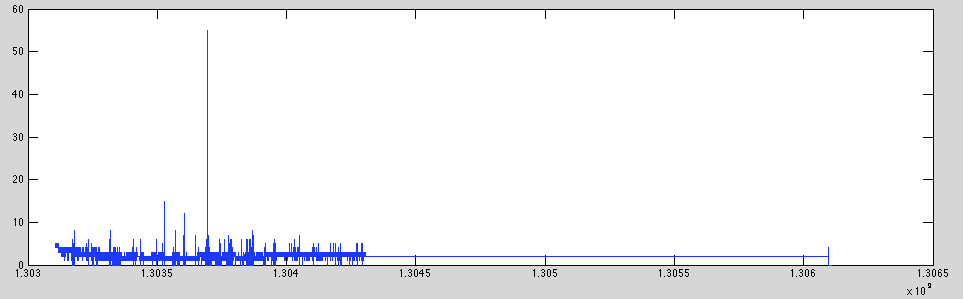
\includegraphics[width=1.0\textwidth,height=0.15\textheight]{channel_7.png}
\caption{washer\_dryer}
\label{fig:washer}
\end{figure*}

\begin{figure*}[th]
\centering
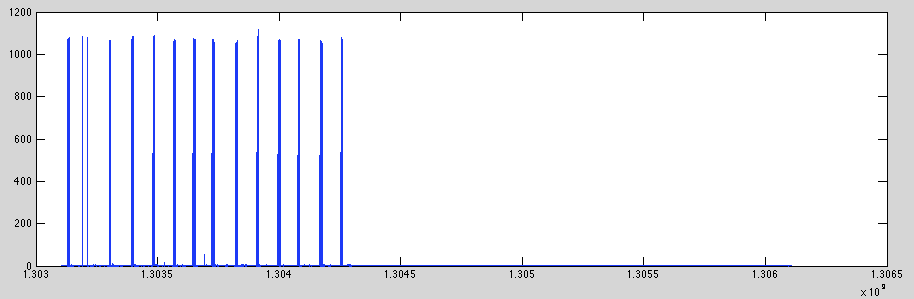
\includegraphics[width=1.0\textwidth,height=0.15\textheight]{channel_8.png}
\caption{Kitchen\_2}
\label{fig:kitchen2}
\end{figure*}

\begin{figure*}[th]
\centering
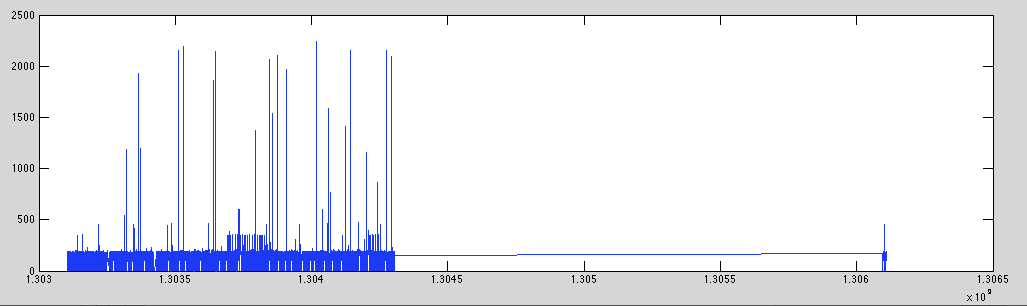
\includegraphics[width=1.0\textwidth,height=0.15\textheight]{channel_9.png}
\caption{refrigerator}
\label{fig:refri}
\end{figure*}

\item \textbf{Code } The implementation of the product of experts model is obtained from Iain Murray's website \cite{code}. It implements the technique described in Geoff Hinton's paper \cite{hinton2000}. 

\item \textbf{Additional details }
Some additional details regarding experiments:
\begin{enumerate}
\item The product of HMMs model (PoHMM) minimizes ``contrastive divergence" as described in the paper \cite{hinton2000}. 
\item The number of experts, $k$ used here is 15. This is set somewhat arbitrarily and needs to be experimented on.
\item Learning rate is $\epsilon = \frac{1}{300}$.
\end{enumerate}
 
\end{itemize}

\section{Experimental Setup}
Experiments are performed on the REDD which contains $9$ appliances each containing $318759$ rows of energy consumption data. Experiments are subdivided into $4$ parts, in the first part the number of data samples are varied corresponding to which the values of KL Divergence and convergence time are noted down. In the second part, the number of experts are varied keeping the best value of the sample from the first part constant. In the third part, number of iterations are varied keeping the best values from part 1 and 2 constant. In the fourth part, the no. of appliances to be aggregated are varied keeping the best values from above parts constant.

\begin{table}[htdp]
\begin{center}
\begin{tabular}{| c | c | c | c |}
\hline
Samples & $KL Div$ & $T(sec)$ & $Iterations$ \\
\hline
300 & 2.4864 & 186.212 $\pm$9.087 & 18600 \\
500 & 0.6761 & 106.564 $\pm$10.046 & 10200 \\
1000 & 1.1088 & 158.521 $\pm$1.97  & 11200 \\
1500 & 3.8829 & 92.896 $\pm$8.075  & 5300 \\
2000 & 1.8686 & 130.98 $\pm$1.932 & 6900 \\
2500 & 0.4733 & 215.563 $\pm$ 2.471 & 9900 \\
3000 & 2.8204 & 258.213 $\pm1.918$ & 11000 \\
3500 & 1.2332 & 204.661 $\pm$1.713 & 7900 \\
4000 & 0.8959 & 292.666 $\pm$0.619 & 10400  \\
4500 & 1.1118 & 222.558 $\pm$1.967 & 7200  \\
8000 & 6.392 & 381.635 $\pm$2.952 & 8100  \\
10000 & 8.276 & 887.932 $\pm$13.824 & 10500  \\
15000 & 0.7201 & 1368.514 $\pm$13.605 & 9400  \\
\hline
\end{tabular}
\end{center}
\caption{Effect of varying samples on KL div and time}
\label{table: error}
\end{table}

\begin{table}[htdp]
\begin{center}
\begin{tabular}{| c | c | c | c |}
\hline
Experts & $KL Div$ & $T(sec)$ & $Iterations$ \\
\hline
5 & 0.774 & 72.968 $\pm$1.177 & 5200 \\
10 & 1.424 & 117.482 $\pm$1.966 & 6700 \\
15 & 0.473 & 210.249 $\pm$1.258  & 9900 \\
20 & 1.56 & 217.739 $\pm$10.452 & 9000 \\
25 & 7.469 & 347.019 $\pm$8.23 & 12100 \\
30 & 2.4968 & 413.802 $\pm$7.304 & 12900 \\
35 & 1.5012 & 348.906 $\pm$14.651 & 11300 \\
\hline
\end{tabular}
\end{center}
\caption{Effect of varying experts on KL div and time}
\label{table: error}
\end{table}


% An example of a floating figure using the graphicx package.
% Note that \label must occur AFTER (or within) \caption.
% For figures, \caption should occur after the \includegraphics.
% Note that IEEEtran v1.7 and later has special internal code that
% is designed to preserve the operation of \label within \caption
% even when the captionsoff option is in effect. However, because
% of issues like this, it may be the safest practice to put all your
% \label just after \caption rather than within \caption{}.
%
% Reminder: the "draftcls" or "draftclsnofoot", not "draft", class
% option should be used if it is desired that the figures are to be
% displayed while in draft mode.
%
%\begin{figure}[!t]
%\centering
%\includegraphics[width=2.5in]{myfigure}
% where an .eps filename suffix will be assumed under latex, 
% and a .pdf suffix will be assumed for pdflatex; or what has been declared
% via \DeclareGraphicsExtensions.
%\caption{Simulation Results}
%\label{fig_sim}
%\end{figure}

% Note that IEEE typically puts floats only at the top, even when this
% results in a large percentage of a column being occupied by floats.


% An example of a double column floating figure using two subfigures.
% (The subfig.sty package must be loaded for this to work.)
% The subfigure \label commands are set within each subfloat command, the
% \label for the overall figure must come after \caption.
% \hfil must be used as a separator to get equal spacing.
% The subfigure.sty package works much the same way, except \subfigure is
% used instead of \subfloat.
%
%\begin{figure*}[!t]
%\centerline{\subfloat[Case I]\includegraphics[width=2.5in]{subfigcase1}%
%\label{fig_first_case}}
%\hfil
%\subfloat[Case II]{\includegraphics[width=2.5in]{subfigcase2}%
%\label{fig_second_case}}}
%\caption{Simulation results}
%\label{fig_sim}
%\end{figure*}
%
% Note that often IEEE papers with subfigures do not employ subfigure
% captions (using the optional argument to \subfloat), but instead will
% reference/describe all of them (a), (b), etc., within the main caption.


% An example of a floating table. Note that, for IEEE style tables, the 
% \caption command should come BEFORE the table. Table text will default to
% \footnotesize as IEEE normally uses this smaller font for tables.
% The \label must come after \caption as always.
%
%\begin{table}[!t]
%% increase table row spacing, adjust to taste
%\renewcommand{\arraystretch}{1.3}
% if using array.sty, it might be a good idea to tweak the value of
% \extrarowheight as needed to properly center the text within the cells
%\caption{An Example of a Table}
%\label{table_example}
%\centering
%% Some packages, such as MDW tools, offer better commands for making tables
%% than the plain LaTeX2e tabular which is used here.
%\begin{tabular}{|c||c|}
%\hline
%One & Two\\
%\hline
%Three & Four\\
%\hline
%\end{tabular}
%\end{table}


% Note that IEEE does not put floats in the very first column - or typically
% anywhere on the first page for that matter. Also, in-text middle ("here")
% positioning is not used. Most IEEE journals/conferences use top floats
% exclusively. Note that, LaTeX2e, unlike IEEE journals/conferences, places
% footnotes above bottom floats. This can be corrected via the \fnbelowfloat
% command of the stfloats package.
\section{Results}
The evaluation of how well the learning has taken place is done by using a Kullback-Leibler divergence metric which gives the difference between two probability distributions. The two probability distributions in the REDD example refer to the expert probabilities in real and fantasy data. The learned parameters from the training are fitted to the fantasy data to measure the information lost when fantasy data is used to approximate real data. This is denoted as D$_{KL}$(real data $|$$|$ fantasy).

\begin{table}[htdp]
\begin{center}
\begin{tabular}{| c | c | c | c |}
\hline
Threshold & $KL Div$ & $T(sec)$ & $Iterations$ \\
\hline
.1 & 0.473 & 210.6 $\pm$1.493 & 9900 \\
.05 & 0.443 & 240.607$\pm$2.436 & 10900 \\
.01 & 0.454 & 431.536 $\pm$14.509 & 18000 \\
.005 & 0.509 & 1167.243 $\pm$43.412 & 49800 \\
\hline
\end{tabular}
\end{center}
\caption{Effect of varying min threshold on KL div and time}
\label{table: error}
\end{table}

\begin{table}[htdp]
\begin{center}
\begin{tabular}{| c | c | c | c |}
\hline
Appliances & $KL Div$ & $T(sec)$ & $Iterations$ \\
\hline
3 & 5.559 & 233.664 $\pm$0.579 & 10700 \\
4 & 0.188 & 465.634 $\pm$5.275 & 19900 \\
5 & .432 & 338.416 $\pm$3.988  & 13400 \\
6 & 8.736 & 606.062 $\pm$7.534 & 28100 \\
7 & 5.054 & 411.457 $\pm$10.051 & 17300 \\
8 & 0.436 & 260.544 $\pm$cc27.862 & 10700 \\
9 & 0.15 & 474.579 $\pm$14.619 & 20600 \\
\hline
\end{tabular}
\end{center}
\caption{Effect of varying appliances on KL div and time}
\label{table: error}
\end{table}

%%This section shows the graphs for different combinations of devices representing how well the learning by product of experts on real data takes place. Experts try to fit the generated data (fantasy data) to the means calculated from the real data. The results of the following pairwise appliances, microwave \& washer, Kitchen$\_$2 \& refrigerator and microwave \& refrigerator are plotted below in Figures~\ref{fig:img1}, ~\ref{fig:img2}, ~\ref{fig:img3}. The black dots represent the fantasy data that is generated from the product of experts. Mean computed by the real data is shown by red dots and ellipses in blue show the one standard deviation contours of the Gaussians in each expert.
%%There are 15 unigauss experts each of which is a mixture of a uniform and a single, axis aligned gaussian. These experts are initialized with randomly located, circular gaussians that have the same variance as the data.
%%In the fitted model, each tight data cluster is represented by the intersection of two gaussians which are elongated along different axes.


\section{Conclusion \& Future Work}
The conclusion goes here. this is more of the conclusion

% conference papers do not normally have an appendix


% use section* for acknowledgement
\section*{Acknowledgment}


The authors would like to thank...
more thanks here


% trigger a \newpage just before the given reference
% number - used to balance the columns on the last page
% adjust value as needed - may need to be readjusted if
% the document is modified later
%\IEEEtriggeratref{8}
% The "triggered" command can be changed if desired:
%\IEEEtriggercmd{\enlargethispage{-5in}}

% references section

% can use a bibliography generated by BibTeX as a .bbl file
% BibTeX documentation can be easily obtained at:
% http://www.ctan.org/tex-archive/biblio/bibtex/contrib/doc/
% The IEEEtran BibTeX style support page is at:
% http://www.michaelshell.org/tex/ieeetran/bibtex/
%\bibliographystyle{IEEEtran}
% argument is your BibTeX string definitions and bibliography database(s)
%\bibliography{IEEEabrv,../bib/paper}
%
% <OR> manually copy in the resultant .bbl file
% set second argument of \begin to the number of references
% (used to reserve space for the reference number labels box)
%\begin{thebibliography}{1}
%
%\bibitem{IEEEhowto:kopka}
%H.~Kopka and P.~W. Daly, \emph{A Guide to \LaTeX}, 3rd~ed.\hskip 1em plus
%  0.5em minus 0.4em\relax Harlow, England: Addison-Wesley, 1999.
%
%\end{thebibliography}

\nocite{hinton2000,code,aistats}

\bibliography{HMM_writeup}
\bibliographystyle{plain}


% that's all folks
\end{document}


